\setcounter{chapter}{-1}
\chapter{What is a matrix?}
%\index{Sample!file}
\begin{chapterquote}[120pt]
�Out of intense complexities intense simplicities emerge.\\
---{\upshape Winston Churchill}\\[6pt]
Three Rules of Work: Out of clutter find simplicity. From discord find harmony. In the middle of difficulty lies opportunity.\\
---{\upshape Albert Einstein}
\end{chapterquote}
\ \\
This preliminary chapter provides a quick review of linear algebra needed to develop the tools command the \svdp. More of the machinery of linear algebra will be developed as we continue to explore the SVD. The goal is to build a basic foundation and to clarify the SVD perspective of linear algebra.

A matrix represents several concepts and the interpretation of a matrix depends upon the context of usage. In terms of the SVD it helps to have a clear understanding of a matrix in terms of the induced vector spaces.

%\begin{algorithm}
%\label{This is a label}
%%\caption{Sample algorithm}
%\begin{algorithmic}
%\IF {$i\geq maxval$} 
%        \STATE $i\gets 0$
%\ELSE
%        \IF {$i+k\leq maxval$}
%                \STATE $i\gets i+k$
%        \ENDIF
%\ENDIF 
%\end{algorithmic}
%\end{algorithm}

%%
\section{Domains}
The concept of a domain comes over very naturally from calculus. A domain is a set of points which defines the set of all valid inputs to a function. Look at the exponential function
\begin{equation}
  y(x) = e^{x}.
\end{equation}
A function is a map: input a variable $x$ and get a variable $y$. The ``$x$ in, $y$ out'' notation will remain even when we switch to linear systems and matrices.
The domain\index{domain!function}, the set of all valid inputs for this function is $\abs{x}<\infty$, the entire real line. We can denote the real line using $\real{1}$. The range\index{range!function} is the set of all function outputs. Here the range is the set of positive definite numbers, $y>0$ denoted as $\real{+}$. This is half of the real line. The exponential function maps numbers from the real line on the positive half of the real line. We may write
\begin{equation}
  y(x)\colon\real{1}\to\real{+}.
\end{equation}
In conversational terms, the function $y(x)$ maps numbers $x$ in the domain $\real{1}$ to values $y$ on the positive half-line $\real{+}$.


The inverse function is the natural logarithm
\begin{equation}
  y^{-1}(x) = \ln (x).
\end{equation}
Here the domain and range are interchanged. The domain is now the positive real numbers $\real{+}$ and the range is the set of all real numbers, $\real{1}$. Here we write
\begin{equation}
  y^{-1}(x)\colon\real{1}\to\real{+}.
\end{equation}

A question to ruminate upon is which function is more fundamental, the exponential or the logarithm? Which is ``the function'' and which is ``the inverse function''? When we think of domains and ranges we see that they interchange under this set of function and inverse. 

The point is that neither function is more fundamental than the other. This means that the assignment of domain and range depend upon the arbitrary choice of whether the exponential is the original function or the inverse function. If we take a pair of functions like the exponential and the logarithm we really can't call one a function and the other an inverse function. They are mutual inverses.

In linear algebra the concept of domain is elaborated upon and we will speak of a domain\index{domain!matrix} and a codomain\index{codomain}. If we take a pair of matrices we really can't call one a matrix and the other a transpose. They are mutual transposes. Therefore the sets of vectors the matrices act upon are a domain and a codomain.

When we looked at functions we saw an example where only part $\real{+}$ of the real line $\real{1}$ was used. If we think of functions as a map we might say that these maps are frustrated because the range did not reach all of the real line, just those numbers greater than zero.

When we jump to linear systems we will see a new wrinkle. Instead of using a \textit{truncation of the real line,} we will use the entire line in \textit{a truncation of dimensionality.}\index{truncation of dimensionality} For example, if the host space were $\real{2}$ we may not use the entire plane. Instead we may be restricted to a line through the origin such as $y(x)=a x$. Of course each point $p$ on this line can be represented as an ordered pair 
\begin{equation}
  p = \mat{c}{x\\y}.
\end{equation}
But we can characterize any any point on the line  with a single scalar $a$ using the distance from the origin.

In this case the host space is $\real{2}$ and the domain is actually the line $\real{1}$. The concept is simple and it highlights an important aspect of the \svdl: sorting out the domains from the host spaces.

Consider the archetypal linear system
\begin{equation}
  \A{}x=y.
\end{equation}
The matrix $\A{}$ multiplies the vector $x$ and produces the vector $y$. The set of all possible vectors $x$ represents the domain. For matrix equations such as this one, the domain will be a class of vectors. The class is defined by the number of free variables in the representation of the vector. For example, the classes with one, two, or three parameters can be represented as
\begin{equation}
\begin{array}{cccc}
  \mat{c}{x_{1}} & \mat{c}{x_{1}\\x_{2}} & \mat{c}{x_{1}\\x_{2}\\x_{3}} & \cdots \\
  \real{1} & \real{2} & \real{3} & \cdots
  \label{eq:1:r}
\end{array}
\end{equation}

The sole restriction on the free parameters $x_{k}$ is that their magnitude is finite: $\abs{x_{k}}<\infty$.

There are distinct ways to reference a point in the domain. Consider a plane. The location 
\begin{equation}
  \mat{c}{\alpha\\\beta} = \alpha \hat{x}_{1} + \beta \hat{x}_{2}  = \alpha \mat{c}{1\\0} + \beta \mat{c}{0\\1},
\end{equation}
with the associations for the unit vectors
\begin{equation}
  \hat{x}_{1} = \mat{c}{1\\0}, \qquad \hat{x}_{2} = \mat{c}{0\\1}.
\end{equation}

To simplify the rendering of figures, we will consider all inputs to be real numbers. Now the examples in equation \eqref{eq:1:r} can be portrayed geometrically as shown in figure \eqref{tab:0:rn}.
%%%%
\begin{table}[htdp]
\begin{center}
\boxed{
\begin{tabular}{{c|c|c}}
    \includegraphics[ width = 1.45in ]{pdf/prelim/r1} &
    \includegraphics[ width = 1.45in ]{pdf/prelim/r2} &
    \includegraphics[ width = 1.45in ]{pdf/prelim/r3} \\\hline
        $\mat{c}{x_{1}}$ & $\mat{c}{x_{1}\\x_{2}}$ & $\mat{c}{x_{1}\\x_{2}\\x_{3}}$\\
        $\real{1}$ & $\real{2}$ & $\real{3}$
\end{tabular}
}
\end{center}
\caption[Domains of increasing dimension, $\real{n}$]{Domains of increasing dimension, $\real{n}$. Here we see representations for a point in $\real{1}$, a line; $\real{2}$, a plane and $\real{3}$, a volume. The axes are mutually orthogonal. Each point in the domain is represented by a $n-$vector $x_{k},\ k=1,n$ which defines a distance from the origin.}
\label{tab:0:rn}
\end{table}%

Every domain has a zero element called the origin. For the examples in equation \eqref{eq:1:r} the origins are
\begin{equation}
\begin{array}{cccc}
  \mat{c}{0}, & \mat{c}{0\\0}, & \mat{c}{0\\0\\0}, & \dots \\
  \real{1} & \real{2} & \real{3} & \dots
  \label{eq:1:r}
\end{array}
\end{equation}
and can be written generally as $\zero$. A very important realization is that \textit{origins are all coincident.} For example if the line $\real{1}$ is embedded in $\real{3}$, the origins represent the same point. For now, we say little about the orientation of the line: in general the unit vectors will not align the line. Think of the free parameters as \textit{coordinates} which describe displacements from the origin.
\endinput
\section{Vectors}
\label{sec:vectors}
Row vectors are fun targets for the \svdl. It's very easy to visualize the domain and codomain.

%%
\subsection{\vv s}
Consider the \vv \ below:
\begin{equation}
  v=\mat{c}{1\\\frac{1}{2}}.
  \label{eq:cases:2v}
\end{equation}
Hopefully the rank of the system is obvious:
\begin{equation}
  \rho = \min\lst{m,n}= \min\lst{2,1} = 1
\end{equation}

The decomposition will have these form factors
\begin{equation}
  \begin{array}{ccccc}
  \A{} &=& \Y{} & \sig{} & \X{T}\\
  \by{m}{n}&=&\paren{\by{m}{m}}&\paren{\by{m}{n}}&\paren{\by{n}{n}}\\
  \by{2}{1}&=&\paren{\by{2}{2}}&\paren{\by{2}{1}}&\paren{\by{1}{1}},
  \end{array}
\end{equation}
as depicted below:
\begin{figure}[htbp] %  figure placement: here, top, bottom, or page
   \centering
   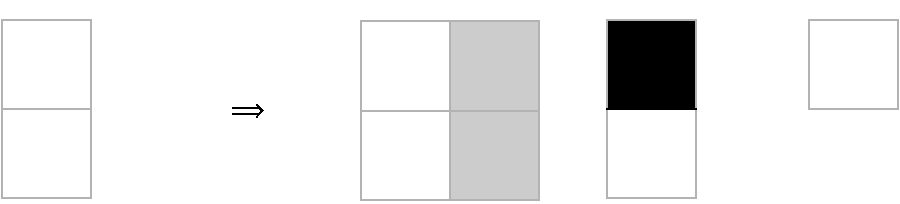
\includegraphics[ width = 4in ]{pdf/more_examples/svd_02_01_01} 
%  ` \caption{example caption}
   \label{fig:examples:21}
\end{figure}

The $\X{}$ matrix is trivial. Since it must be unitary the magnitude is one:
\begin{equation}
  \X{}= \mat{c}{1}.
\end{equation}
The lone singular value is the scale factor $r=\sqrt{2^{2}+\frac{1}{2}^{2}}$ which is the length of the vector:
\begin{equation}
  \sig{} = \mat{c}{\frac{\sqrt{5}}{2}\\0}.
\end{equation}
  For the codomain matrix we start with the image and normalize the column vector:
\begin{equation}
  \Y{}=\mat{cc}{c_{1}&c_{2}}, \qquad c_{1}=\frac{\sqrt{5}}{2}\mat{c}{2\\1}.
\end{equation}
The only quantity missing now is the null space vector $c_{2}$. Pick an orthogonal complement to $c_{1}$ and the codomain basis matrix is
\begin{equation}
  \Y{}=\frac{1}{\sqrt{5}}\mat{rr}{2&1\\1&-2}.
\end{equation}
The \svdl \ is then
\begin{equation}
  \begin{split}
    \svda{T}\\
    \mat{c}{1\\\frac{1}{2}} &= \frac{1}{\sqrt{5}}
    \mat{rr}{2&-1\\1&2}
    \mat{c}{\frac{\sqrt{5}}{2}\\0}
    \mat{c}{1}.
  \end{split}
  \label{eq:cases:2vdecomp}
\end{equation}

%%
\subsection{\vvv s}
Consider this \vvv:
\begin{equation}
  v = \mat{r}{1\\2\\-2}.
\end{equation}
The decomposition will have the shapes given by this
\begin{equation}
  \begin{array}{ccccc}
  \A{} &=& \Y{} & \sig{} & \X{T}\\
  \by{m}{n}&=&\paren{\by{m}{m}}&\paren{\by{m}{n}}&\paren{\by{n}{n}}\\
  \by{3}{1}&=&\paren{\by{3}{1}}&\paren{\by{3}{1}}&\paren{\by{1}{1}},
  \end{array}
\end{equation}
as shown here:
\begin{figure}[htbp] %  figure placement: here, top, bottom, or page
   \centering
   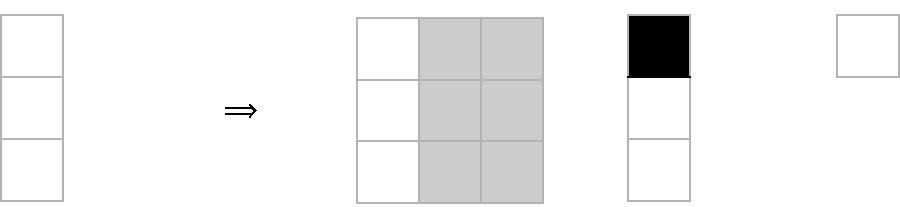
\includegraphics[ width = 4in ]{pdf/more_examples/svd_03_01_01} 
%   \caption{example caption}
   \label{fig:examples:31}
\end{figure}

We can use this vector to seed the codomain matrix:
\begin{equation}
  \Y{}_{*,1} = \frac{1}{3}\mat{r}{1\\2\\-2}.
\end{equation}
This leaves the null space vectors. A first candidate is 
\begin{equation}
  \Y{}_{*,2} = \frac{1}{\sqrt{2}}\mat{r}{0\\1\\1}.
\end{equation}
Using an inspection-based algorithm we can pick a vector like
\begin{equation}
  \Y{}_{*,3} = \frac{1}{\sqrt{18}}\mat{r}{4\\-1\\1}.
\end{equation}
The lone singular value is the length of the vector. The \svdl \ becomes
\begin{equation}
  \begin{split}
    \svda{T}\\
    \mat{r}{1\\2\\-2} &=
    \left[
\begin{array}{ r >{\columncolor{ltgray}}r >{\columncolor{ltgray}}r }
  \frac{1}{3} & 0 & \frac{4}{ \sqrt{18} } \\[5pt]
  \frac{2}{3} & \frac{1}{\sqrt{2}} & -\frac{1}{ \sqrt{18} } \\[5pt]
 -\frac{2}{3} & \frac{1}{\sqrt{2}} &  \frac{1}{ \sqrt{18} }
\end{array}
\right] 
    \left[
\begin{array}{c}
 3 \\ \hline
 0 \\
 0
\end{array}
\right]
  \mat{c}{1}.
  \end{split}
\end{equation}

The shortcut won't work. 
\begin{equation}
  v = \mat{c}{\sin\theta \\ 0 \\ \cos\theta}.
\end{equation}

\begin{equation}
  \begin{split}
    \W{y} = v v^{\mathrm{T}} &= \mat{c}{\sin\theta \\ 0 \\ \cos\theta}\mat{ccc}{\sin\theta & 0 & \cos\theta}\\
    &= \mat{ccc}{\sin^{2}\theta & 0 & \sin\theta \cos\theta\\ 0 & 0 & 0 \\ \sin\theta \cos\theta & 0 & \cos^{2}\theta}
  \end{split}
\end{equation}


Characteristic polynomial
Use cofactor expansion to compute the determinant
\begin{equation}
  \begin{split}
    p(\lambda) &= \det \paren{\W{y} - \lambda \I{3}}\\ &= 
    \det\mat{c|r|c}{\sin^{2}\theta - \lambda & 0 & \sin\theta \cos\theta\\\hline 0 & - \lambda & 0 \\ \sin\theta \cos\theta & 0 & \cos^{2}\theta- \lambda} \\
    &= \paren{\sin^{2}\theta - \lambda}\det\mat{cc}{-\lambda & 0 \\ 0 & \cos^{2}\theta- \lambda}\\ & \quad- 0 \det\mat{cc}{0 & 0 \\ \sin\theta \cos\theta & \cos^{2}\theta- \lambda}\\
     & \quad + \paren{\cos^{2}\theta - \lambda}\det\mat{cc}{0 & -\lambda \\ \sin\theta \cos\theta & 0}\\
  \end{split}
\end{equation}

The roots of the characteristic polynomial are the eigenvalues
\begin{equation}
  p(\lambda) = \lambda^{2}\paren{\lambda-1} = 0
\end{equation}
leads to the spectrum
\begin{equation}
  \lambda\paren{\W{y}} = \lst{1,0,0}.
\end{equation}
Therefore there is one singular value, 
\begin{equation}
  \sigma_{1} = 1.
\end{equation}
The eigenvector solves
\begin{equation}
  \begin{split}
    \W{y}u &= \lambda u\\
    \mat{ccc}{\sin^{2}\theta & 0 & \sin\theta \cos\theta\\ 0 & 0 & 0 \\ \sin\theta \cos\theta & 0 & \cos^{2}\theta} \mat{c}{u_{1} \\ 0 \\ u_{3}} & = \mat{c}{u_{1} \\ 0 \\ u_{3}}
  \end{split}
\end{equation}
This reduces to the system
\begin{equation}
\mat{cc}
{\sin^{2}\theta & \sin\theta \cos\theta\\
 \sin\theta \cos\theta & \cos^{2}\theta}
\mat{c}{u_{1} \\ u_{3}} = \mat{c}{u_{1} \\ u_{3}}
\end{equation}



%%
\subsection{$10-$vectors}
You can quickly verify that
\begin{equation}
  \begin{split}
    \svda{T}\\
    \mat{r}{1\\0\\0\\0\\0\\0\\0\\0\\0\\0} &=
    \left[
\begin{array}{ r >{\columncolor{ltgray}}r >{\columncolor{ltgray}}r >{\columncolor{ltgray}}r >{\columncolor{ltgray}}r >{\columncolor{ltgray}}r >{\columncolor{ltgray}}r >{\columncolor{ltgray}}r >{\columncolor{ltgray}}r >{\columncolor{ltgray}}r }
  1 & 0 & 0 & 0 & 0 & 0 & 0 & 0 & 0 & 0 \\
  0 & 1 & 0 & 0 & 0 & 0 & 0 & 0 & 0 & 0 \\
  0 & 0 & 1 & 0 & 0 & 0 & 0 & 0 & 0 & 0 \\
  0 & 0 & 0 & 1 & 0 & 0 & 0 & 0 & 0 & 0 \\
  0 & 0 & 0 & 0 & 1 & 0 & 0 & 0 & 0 & 0 \\
  0 & 0 & 0 & 0 & 0 & 1 & 0 & 0 & 0 & 0 \\
  0 & 0 & 0 & 0 & 0 & 0 & 1 & 0 & 0 & 0 \\
  0 & 0 & 0 & 0 & 0 & 0 & 0 & 1 & 0 & 0 \\
  0 & 0 & 0 & 0 & 0 & 0 & 0 & 0 & 1 & 0 \\
  0 & 0 & 0 & 0 & 0 & 0 & 0 & 0 & 0 & 1 \\
\end{array}
\right] 
    \left[
\begin{array}{c}
 1 \\ \hline
 0 \\
 0 \\
 0 \\
 0 \\
 0 \\
 0 \\
 0 \\
 0 \\
 0
\end{array}
\right]
  \mat{c}{1}.
  \end{split}
\end{equation}

This is such a simple exercise because the column vectors are already unit vectors.

A Givens rotation by an angle $\theta$ in the $4-8$ plane does not affect the decomposition because the codomain matrix $\Y{}$ is still orthogonal
\begin{equation}
  \Y{'} = 
      \left[
\begin{array}{ c >{\columncolor{ltgray}}c >{\columncolor{ltgray}}c >{\columncolor{ltgray}}c >{\columncolor{ltgray}}c >{\columncolor{ltgray}}c >{\columncolor{ltgray}}c >{\columncolor{ltgray}}c >{\columncolor{ltgray}}c >{\columncolor{ltgray}}c }
  1 & 0 & 0 & 0 & 0 & 0 & 0 & 0 & 0 & 0 \\
  0 & 1 & 0 & 0 & 0 & 0 & 0 & 0 & 0 & 0 \\
  0 & 0 & 1 & 0 & 0 & 0 & 0 & 0 & 0 & 0 \\
  0 & 0 & 0 & \cos \theta & 0 & 0 & 0 & -\sin \theta & 0 & 0 \\
  0 & 0 & 0 & 0 & 1 & 0 & 0 & 0 & 0 & 0 \\
  0 & 0 & 0 & 0 & 0 & 1 & 0 & 0 & 0 & 0 \\
  0 & 0 & 0 & 0 & 0 & 0 & 1 & 0 & 0 & 0 \\
  0 & 0 & 0 & \sin \theta & 0 & 0 & 0 & \cos \theta & 0 & 0 \\
  0 & 0 & 0 & 0 & 0 & 0 & 0 & 0 & 1 & 0 \\
  0 & 0 & 0 & 0 & 0 & 0 & 0 & 0 & 0 & 1 \\
\end{array}
\right] 
\end{equation}

Yet another rotation 1-9:
\begin{equation}
  \Y{'} = 
      \left[
\begin{array}{ c >{\columncolor{ltgray}}c >{\columncolor{ltgray}}c >{\columncolor{ltgray}}c >{\columncolor{ltgray}}c >{\columncolor{ltgray}}c >{\columncolor{ltgray}}c >{\columncolor{ltgray}}c >{\columncolor{ltgray}}c >{\columncolor{ltgray}}c }
  \cos \phi & 0 & 0 & 0 & 0 & 0 & 0 & 0 & -\sin \phi & 0 \\
  0 & 1 & 0 & 0 & 0 & 0 & 0 & 0 & 0 & 0 \\
  0 & 0 & 1 & 0 & 0 & 0 & 0 & 0 & 0 & 0 \\
  0 & 0 & 0 & \cos \theta & 0 & 0 & 0 & -\sin \theta & 0 & 0 \\
  0 & 0 & 0 & 0 & 1 & 0 & 0 & 0 & 0 & 0 \\
  0 & 0 & 0 & 0 & 0 & 1 & 0 & 0 & 0 & 0 \\
  0 & 0 & 0 & 0 & 0 & 0 & 1 & 0 & 0 & 0 \\
  0 & 0 & 0 & \sin \theta & 0 & 0 & 0 & \cos \theta & 0 & 0 \\
  \sin \phi & 0 & 0 & 0 & 0 & 0 & 0 & 0 & \cos \phi & 0 \\
  0 & 0 & 0 & 0 & 0 & 0 & 0 & 0 & 0 & 1 \\
\end{array}
\right] 
\end{equation}


\endinput
\section{Matrices}
For clarity matrices are typeset in emboldened letters. Throughout this book we will be considering matrices in general as a collection of complex numbers with $m$ rows and $n$ columns. The height of the matrix is determined by $m$, the number of rows; the width by $n$ the number of columns. The important point is that the number of rows are specified first, then the number of columns:
\begin{equation}
  \paren{\by{rows}{columns}}=\paren{\by{m}{n}}.
\end{equation}
The first row is the top row and the first column is the left-most column.

Formally we specify a matrix as
\begin{equation}
  \A{}\in\cmplx{\by{m}{n}}
\end{equation}
even if only one entry is complex. If all matrix entries are real we instead write
\begin{equation}
  \A{}\in\real{\by{m}{n}}.
\end{equation}
It is not so much the collection of numbers that is of interest here as the meaning of the rows and columns. But other properties require explanation first.

%%
\subsection{Matrix rank}
A critical matrix property is rank\index{rank!matrix}, denoted here by the parameter $\rho$.  The rank details the number of independent rows or columns. You may speak of row rank\index{rank!row}, the number of independent rows, or column rank\index{rank!column}, the number of independent columns. However the matrix rank is the same as the row rank and the same as the column rank. 
$$
\text{matrix rank} = \text{row rank} = \text{column rank}.
$$
Below are some examples of $\bys{3}$ matrices of different ranks in reduced form.
\begin{equation}
\begin{array}{ccc}
\mat{rcr}
{
-2 & e^{-1} & 1\\
 0 &  i & 0\\
 0 &  0 &-4
}, \qquad & 
\mat{ccc}
{
 1 &  2i & 0\\
 0 &  8 & \pi\\
 0 &  0 & 0
}, \qquad & 
\mat{rrc}
{
\sqrt[4]{2} & -1 & \pi^{2}\\
 0 &  0 & 0\\
 0 &  0 & 0
} \\[5pt]
\rho = 3 & \rho = 2 & \rho = 1
\end{array}
\end{equation}

Certainly then the rank can be no larger than the minimum of the dimension parameters $m$ and $n$. That is
\begin{equation}
  \rho \le \min \lst{m,n}.
\end{equation}
To include the rank in the matrix specification use a subscript as shown here
\begin{equation}
  \A{}\in\cmplx{\by{m}{n}}_{\rho}.
\end{equation}

For example, consider a matrix with three rows, but only two are linearly independent. The second row is equal to two times the first row minus the third row. This matrix is
\begin{equation}
  \A{}\in\cmplx{\by{3}{columns}}_{2} = \mat{c}
  {
  r_{1}\\ \hline
  2r_{1}-r_{3}\\ \hline
  r_{3}
  }.
\end{equation}
Because there are two linearly independent rows, row 1 and row 3, the row rank of this matrix is $\rho = 2$. Therefore the matrix rank is also two. Notice that the number of columns must be $n \ge \rho$. 

The same principle applies to the columns. Here is a matrix where the first column is the sum of last three columns. This matrix is
\begin{equation}
  \A{}\in\cmplx{\by{rows}{4}}_{3} = \mat{c|c|c|c}
  {
  c_{2}+c_{3}-c_{4} & c_{2} & c_{3} & c_{4}
  }.
\end{equation}
Because there are three linearly independent columns, rows 2, 3, and 4, the column rank of this matrix is $\rho = 3$. Therefore the matrix rank is also three. The number of rows must be $m \ge \rho$.

The matrices generated by the outer product are all rank one matrices as shown by equation \eqref{prelim:vectors:outer}. Each row is a multiple of the input row vector.

The concept of matrix rank is a rich one which will prove invaluable. Further explanation is deferred.

%%
\subsection{Matrix multiplication}
There are a few ways to address matrix multiplication\index{matrix!multiplication}. The paradigm of interest here is to cast matrix multiplication as a series of dot products between row vectors and column vectors. For the matrix equation
\begin{equation}
  \begin{array}{cccc}
  \A{}&\B{} &=& \C{}\\
  \paren{\by{m}{p}} & \paren{\by{p}{n}} && \paren{\by{m}{n}}
  \end{array}
  \label{eq:mprod}
\end{equation}
the element of the product matrix $\C{}$ in row $r$ and column $c$ is given by the dot product of the $r$th row of $\A{}$ with the $c$th column of $\B{}$. The result is the scalar $\C{}_{r,c}$. This equation may simpler to understand than the words:
\begin{equation}
  \C{}_{r,c} = \underbrace{\A{}_{r,*}}_{\text{row }r}\cdot\underbrace{\B{}_{*,c}}_{\text{col }c}.
  \label{eq:dot}
\end{equation}
An schematic example is shown in figure \eqref{fig:1:mmult} where $\C{}_{2,4} = \A{}_{2,*}\cdot\B{}_{*,4}.$
%%%
\begin{figure}[htbp] %  figure placement: here, top, bottom, or page
   \centering
   \includegraphics[]{pdf/prelim/multiply.pdf} 
   \caption[Each entry in a product matrix is computed as a dot product]{Each entry in a product matrix is computed as a dot product. Row vectors on the left matrix are dotted with column vectors in the right matrix. The concept of conformability for $\A{}\B{}=\C{}$ is distinctly shown here as both vectors must have the same length.}
   \label{fig:1:mmult}
\end{figure}
%%%
The dot product rule dictates the conformability condition\index{conformability condition}. For a product matrix of dimension $\by{m}{n}$ the component matrices must have the dimensions
of $\by{m}{p}$ for the left matrix and $\by{p}{n}$ for the right matrix as shown in equation \eqref{eq:mprod} and emphasized here
\begin{equation}
\paren{\by{m}{p}}\paren{\by{p}{n}}=\by{m}{n}.
\end{equation}
The crucial observation is that the vectors in the dot product have common dimension $p$.

Because it is easy to confuse the convention\footnote{Meyer has a very nice explanation of the source of the convention in his book, \cite[p. 123]{Meyer}.} an example follows. Think of an example of two matrices multiplied in different orders. Take a wide matrix that is $m \times n = 2\times5$ and a tall matrix that is $5\times 2$. Multiply wide by tall, then tall by wide and look at the shape of the product matrices. This realization will be recalled in the section on product matrices,
%%%
\begin{figure}[htbp] %  figure placement: here, top, bottom, or page
\includegraphics[ width = 3.75in ]{pdf/prelim/mult_prods}\\
   \caption[Shape dynamics]{Shape dynamics. The product matrix inherits the height from the matrix on the left, the width from the matrix on the right. That is height from the left, width from the right.}
   \label{fig:example}
\end{figure}
%%%
%%
\subsection{The matrix transpose}
The matrix transpose appears over and over throughout linear algebra and is a generalization of vector transposition.

Taking the transpose of a matrix means interchanging the rows and columns. Row 1 becomes column 1, row 2 becomes column 2, and so on. The rule has the result
\begin{equation}
  \begin{split}
    \A{}&\in\cmplx{\by{m}{n}},\\
    \A{T}&\in\cmplx{\by{n}{m}},
  \end{split}
\end{equation}
showing the interchange of $m$ and $n$.

If $\A{}$ had $m=5$ rows and $n=2$ columns the transpose $\A{T}$ will have $m=2$ rows and $n=5$ columns. 
Taking the transpose of the transpose restores the target matrix to original form. That is,
\begin{equation}
  \paren{\A{T}}^{\mathrm{T}}=\A{}.
\end{equation}

An elementary exercise, e.q. \cite[p. 10]{Meyer}, \cite[p. 8]{Strang}, shows the reverse order rule for matrix products:
\begin{equation}
  \paren{\A{}\B{}}^{\mathrm{T}}=\B{T}\A{T}.
  \label{eq:mattran}
\end{equation}

Philosophically, neither matrix nor transpose is a more fundamental object than the other. Certainly in terms of a specific computation there will be a preference flowing from the association with the rows and columns. But without an association to a measurement system, a matrix and its transpose share equivalence. Ultimately this lack of ascendancy will lead to the concept of domain and codomain.

%%
\subsection[Matrices do not commute]{Matrices do not commute under multiplication}
Matrices share many properties with scalars like associativity and distributivity. But matrices do not commute in general. That is typically
\begin{equation}
  \brac{\A{},\B{}} = \A{}\B{}-\B{}\A{} \ne \zero.
  \label{eq:matcom}
\end{equation}

A quick way to realize this is to imagine a rectangular matrix where $m\ne n$. The product matrix $\A{}\A{T}$ is a square matrix of dimensions $\by{m}{m}$ and the product matrix $\A{T}\A{}$ is a square matrix of dimensions $\by{n}{n}$. We cannot difference these matrices of different sizes.

What if the problem is restricted to the class of square matrices where $m=n$? Then the issue is that we are using \textit{different vectors} in the dot products. Rewrite \eqref{eq:matcom} as 
\begin{equation}
  \brac{\A{},\B{}} = \A{}\B{}-\B{}\A{} = \overrightarrow{\C{}} - \overleftarrow{\C{}}
\end{equation}
and consider the matrix elements 
\begin{equation}
  \begin{split}
    \overrightarrow{\C{}}_{r,c} &= \A{}_{r,*}\cdot\B{}_{*,c},\\
    \overleftarrow{\C{}}_{r,c} &= \B{}_{r,*}\cdot\A{}_{*,c}.\\
  \end{split}
\end{equation}
In general
\begin{equation}
   \overrightarrow{\C{}}_{r,c} \ne \overleftarrow{\C{}}_{r,c}
\end{equation}
because
\begin{equation}
  \A{}_{r,*}\cdot\B{}_{*,c} \ne \B{}_{r,*}\cdot\A{}_{*,c}.
\end{equation}
The issue is that in one direction, $\A{}\B{}$, we are using the \textit{row} vectors of $\A{}$. The other direction, $\B{}\A{}$, involves the \textit{column} vectors of $\A{}$. Clearly, the general matrix does not enforce an equality between row and column vectors.

%%
\subsection{The adjoint}
One of the most important operations we will perform on a matrix is the \textit{adjoint}\index{adjoint} operation, also called \index{Hermitian conjugation}\textit{Hermitian conjugation.} This interchanges the rows and columns and requires that we take the complex conjugate of each matrix entry. If $a_{r,c}$ is the element in row $r$ and column $c$ the matrix $\A{}$ then we can symbolically represent this process as 
\begin{equation}
  \begin{split}
    \A{} &\to \A{*}\\
    a_{r,c} &\to \overline{a}_{c,r}
  \end{split}
\end{equation}

The complex conjugate of this element will appear in row $c$ and column $r$ in the matrix $\A{*}$.

When working with complex matrices
\begin{equation}
    \A{*}= \overline{\A{}}^{\mathrm{T}}= \overline{\A{T}}.
\end{equation}
The operations of conjugation and transposition commute; that is, they can be performed in any order as shown above.

Quite often we will restrict our attention to the field of real numbers and dispense with the generality of the complex field. In these cases the adjoint is the transpose.

%%
\subsection{Product matrices}
Product matrices are an important topic for this book. In general the matrices that we study are not square which makes it impossible to discuss important properties like eigenvalues. To extend these concepts to rectangular matrices, form either of the square matrices
\begin{equation}
  \begin{split}
    \W{x} &= \prdm{*}, \\
    \W{y} &= \prdmm{*}.
    \label{eq:prelim:w}
  \end{split}
\end{equation}
The astute reader may wonder about the assignment of the subscripts for the product matrices. The convention is rudimentary:
\begin{enumerate}
\item $\W{x}\in\cmplx{\by{n}{n}}$ and is conformable with $n-$vectors from the \textit{domain};
\item $\W{y}\in\cmplx{\by{m}{m}}$ and is conformable with $m-$vectors from the \textit{codomain}.
\end{enumerate}
This foreshadows the richer context of matrix domain.

While the term ``product matrix'' has the general connotation as in equation \eqref{eq:mprod}, in this work ``product matrices'' implies $\W{x}$ and $\W{y}$, the two situations where a matrix is multiplied with its adjoint.

%%
\subsection{Left and right operations}
A recurring theme in this book are left and right operations on matrices. 
The usual condition is when the target matrix premultiplies a vector as in 
\begin{equation}
\A{}x=y.
\label{eq:axy}
\end{equation}
Another option is postmultiplication of the vector by the matrix. This can be expressed by premultiplication of the transpose matrix upon the vector transpose:
\begin{equation}
  \paren{y^{\mathrm{T}}\A{}}^{\mathrm{T}} = \A{T}y=x.
\label{eq:ayx}
\end{equation}
These last two statements have deep implications. We see that the target matrix operates on an $n-$vector $x$ and returns an $m-$vector $y$. Also, the transpose matrix operates on an $m-$vector $y$ and returns an $n-$vector $x$. (Please be very clear that the vector pairs $(x,y)$ in \eqref{eq:axy} are different from the vector pairs $(x,y)$ in \eqref{eq:ayx}. The transpose is not an inverse; the transpose always exists, the inverse sometimes so.)

We saw that matrices operate upon column vectors on the right and that row vectors on the left operate upon matrices.

When we examine the pseudoinverse, the generalized matrix inverse, we will that every matrix $\A{}$ has a pseudoinverse $\A{+}$. In some cases this will be a left inverse
\begin{equation}
  \leftinv = \I{n},
\end{equation}
in other cases it may be a right inverse
\begin{equation}
  \rightinv = \I{m}.
\end{equation}
In the first case premultiplication by the pseudoinverse produced an identity matrix. In the second case postmultiplication produced an identity matrix.

%%
\subsection{Domain and codomain}
A matrix is a map between two vector spaces, the space of $m-$vectors and the space of $n-$vectors. So both spaces are domains. By convention the space of $n-$vectors is called the \index{domain and codomain}\textit{domain} and the space of $m-$vectors is called the \index{codomain}\textit{codomain}. Therefore neither domain nor codomain is a more fundamental object.

Going back we can read this equation
\begin{equation*}
  \A{}x=y
\end{equation*}
as ``The matrix $\A{}$ maps $n-$vectors in the domain $X$ to $m-$vectors in the codomain $Y$.''
We can read the equation
\begin{equation*}
  \A{*}y=x
\end{equation*}
as ``The adjoint matrix $\A{*}$ maps $m-$vectors in the codomain $Y$ to $n-$vectors in the domain $X$.''

More formally, the vector space $X$ is the set of all vectors of length $n$. Of course then the vector space $Y$ is the set of all vectors of length $m$.

To close this section we present a summary table.
%%%
\begin{table}[htdp]
\begin{center}
\begin{tabular}{llcl}
  matrix & maps from  && maps to \\\hline
  $\A{}$ & domain   & $\mapsto$ & codomain \\
         & \mv s    & $\mapsto$ & \nv s \\
         & $X$      & $\mapsto$ & $Y$    \\[3pt]
  $\A{*}$& codomain & $\mapsto$ & domain \\
         & \nv s    & $\mapsto$ & \mv s \\
         & $Y$      & $\mapsto$ & $X$    
\end{tabular}
\end{center}
\label{tab:00:mappings}
\caption{Matrix mapping actions. Here $\Accmn$ and we see how the matrix and it adjoint maps between the domain and the codomain.}
\end{table}%


%%
\subsection{The range of a matrix}
A bedrock concept of linear algebra is the \textit{range}\index{range} of a matrix. The range of a matrix $\A{}$ is the collection of all possible $m-$vectors generated by the matrix $\A{}$ when acting upon $n-$vectors:
\begin{equation}
  \rng{\A{}}=\lst{\A{}x\colon x \in \cmplx{n}}\subseteq \cmplx{m}.
\end{equation}

For example the range of the identity matrix
\begin{equation}
  \I{2}=\mat{cc}{1&0\\0&1}
\end{equation}
is the entire plane $\real{2}$. Any point in the plane can be reached with the appropriate $x$ vector. The arbitrary point 
\begin{equation}
  p = \mat{c}{\alpha \\ \beta}
\end{equation}
can be reached by using the vector
\begin{equation}
  x = \mat{c}{\alpha \\ \beta}
\end{equation}
since 
\begin{equation}
  \A{} x = p.
\end{equation}

However for matrices that do not have full rank there will always be restrictions on the range. It will not be $\real{m}$. The matrix
\begin{equation}
  \A{}=\mat{cc}{1&0\\0&0}
\end{equation}
can only produce vectors on the $x-$axis. There are no vectors which map to the any point with a non-zero $y-$coordinate. For example, there exists no such vector $x$ which solves 
\begin{equation}
  \A{}x=\mat{cc}{1&0\\0&0}\mat{c}{x_{1}\\x_{2}} = \mat{c}{0\\1}.
\end{equation}

The geometric interpretation of range\index{range!geometric interpretation} leads to the a different perspective of matrix actions upon vectors. When a matrix acts upon a vector the result is a linear combination of the column vectors of the matrix as shown below:
\begin{equation}
\begin{split}
  \A{}x&=\mat{c|c|c|c}{\A{}_{*,1} & \A{}_{*,2} & \A{}_{*,3} & \hdots}\mat{c}{x_{1} \\ x_{2} \\ x_{3} \\ \vdots} \\
    &= x_{1} \A{}_{*,1} + x_{2} \A{}_{*,2} + x_{3} \A{}_{*,3} + \dots .
\end{split}
\end{equation}
In this context, the range of a matrix is all possible linear combinations of the column vectors. Since this concept can also be framed as all possible combinations of the column vectors, the range is sometimes called the image space\index{image space} (or image) of a matrix.

%%
\subsection{The condition number}
The condition number, $\kappa$, is one of the most important diagnostic quantities we have for a matrix. It is a measure of the precision of the inverse mapping. A simple example illustrates the point. Examine the matrix sequence
\begin{equation}
\begin{array}{ccccc}
  \mat{cc}{1&0\\0&1} & \to & \mat{cc}{1&0\\0&\epsilon} & \to & \mat{cc}{1&0\\0&0}\\[15pt]
  \kappa = 1 && \kappa = 1/\epsilon && \kappa = \infty.
\end{array}
\end{equation}
The matrix on the left, the identity matrix has the ideal condition number of unity. The matrix on the right is rank-deficient and has infinite condition number. The matrix in the middle has ambiguous condition number and we see that as the parameter $\epsilon$ varies from 1 to 0 the conditioning goes from ideal to disasterous. In fact, one would certainly suspect that as $\epsilon$ nears the machine epsilon of your computer computations involving this matrix will be unreliable.

A more formal definition will follow later because the emphasis here is on intuition. For now consider three basic cases:
\begin{enumerate}
\item The ideal case, $\kappa=1$, for exact maps like identity matrices. This means that all vectors $\paren{y_{1},y_{2}}^{\mathrm{T}}$ in the codomain  can be exactly mapped to all source vectors $\paren{x_{1},x_{2}}^{\mathrm{T}}$ in the domain by the matrix inverse.
\item Imprecise maps where the condition number is large. Some vectors $\paren{y_{1},y_{2}}^{\mathrm{T}}$ in the codomain may be mapped by the inverse not to the source vector $\paren{x_{1},x_{2}}^{\mathrm{T}}$, but instead to a nearby vector.
\item Frustrated maps where $\kappa=\infty$. Entire classes of vectors $\paren{y_{1},y_{2}}^{\mathrm{T}}$ in the codomain cannot be mapped to any vectors in the domain $\paren{x_{1},x_{2}}^{\mathrm{T}}$.
\end{enumerate}

%%
\subsection{A note on terminology}
Basic terminology differences distinguish between real and complex matrices. If all entries in a matrix are real, then the matrix is real. If at least one matrix entry is imaginary or complex, then the matrix is complex. Many texts avoid stirring complex numbers into the mix. The philosophy here is that the added intricacy of complex arithmetic is more than offset by the unique properties we will explore in the complex realm.

The table below shows the differences in terminology between real and complex matrices.
\begin{equation}
\boxed{
\begin{array}{cc}
  \text{real matrices} & \text{complex matrices} \\\hline\hline
  \text{transpose} & \text{adjoint} \\
  \A{T} & \A{*} \  \paren{= \overline{\A{T}}} \\[10pt]\hline
  \text{orthogonal} & \text{unitary} \\
  \A{-1}=\A{T} & \A{-1}=\A{*}
\end{array}
}
\end{equation}

The complex notation is more general and should be used if the matrix entries are not restricted to be real numbers. However if all matrix entries are real the custom is to use notation for real matrices. 

\endinput
% bys
\newcommand{\by}[2]      {#1 \times #2}
\newcommand{\byy}[1]     {#1 \times #1}
\newcommand{\bymn}[0]    {\by{m}{n}}
\newcommand{\bymm}[0]    {\byy{m}}
\newcommand{\bynn}[0]    {\byy{n}}
\newcommand{\bynm}[0]    {\by{n}{m}}
\newcommand{\bymr}[0]    {\by{m}{\rho}}
\newcommand{\byrn}[0]    {\by{\rho}{n}}

% vector spaces
\newcommand{\real}[1]    {\mathbb{R}^{#1}}
\newcommand{\cmplx}[1]   {\mathbb{C}^{#1}}
\newcommand{\either}[1]  {\cmplx{#1}}
\newcommand{\ir}[0]      {\in\real{}}
\newcommand{\ic}[0]      {\in\cmplx{}}
\newcommand{\icm}[0]     {\in\cmplxm}
\newcommand{\icn}[0]     {\in\cmplxn}
\newcommand{\icmn}[0]    {\in\cmplxmn}
\newcommand{\irmn}[0]    {\in\realmn}
\newcommand{\icmnr}[0]   {\in\cmplxmnr}
\newcommand{\ints}[0]    {\mathbb{Z}}
\newcommand{\natnum}[0]  {\mathbb{N}}

\newcommand{\iints}[0]   {\in \mathbb{Z}}
\newcommand{\inatnum}[0] {\in \mathbb{N}}

\newcommand{\realall}[3] {\real{\by{#1}{#2}}_{#3} }
\newcommand{\cmplxall}[3]{\cmplx{\by{#1}{#2}}_{#3} }

\newcommand{\realn}[0]   {\real{n}}
\newcommand{\realm}[0]   {\real{m}}
\newcommand{\realmn}[0]  {\real{\bymn}}
\newcommand{\realnn}[0]  {\real{\byy{n}}}
\newcommand{\realmm}[0]  {\real{\byy{m}}}
\newcommand{\realmmr}[0] {\real{\byy{m}}_{\rho}}
\newcommand{\realmmm}[0] {\realmm_{m}}

\newcommand{\cmplxn}[0]  {\cmplx{n}}
\newcommand{\cmplxm}[0]  {\cmplx{m}}
\newcommand{\cmplxnn}[0] {\cmplx{\byy{n}}}
\newcommand{\cmplxmm}[0] {\cmplx{\byy{m}}}
\newcommand{\cmplxmn}[0] {\cmplx{\bymn}}
\newcommand{\cmplxmr}[0] {\cmplx{\bymr}}
\newcommand{\cmplxrn}[0] {\cmplx{\byrn}}
\newcommand{\cmplxmnr}[0]{\cmplx{\bymn}_{\rho}}
\newcommand{\cmplxmmm}[0]{\cmplxmm_{m}}
\newcommand{\cmplxmnm}[0]{\cmplxmn_{m}}
\newcommand{\cmplxnnr}[0]{\cmplxnn_{\rho}}
\newcommand{\cmplxmnn}[0]{\cmplxmn_{n}}

% spans
\newcommand{\spn}[1]     {\text{sp\,} \lst{ #1 }}


\endinput  %  -  -  -  -  -  -  -  -  -  -  -  -  -  -  -  -  -  -  -  -
\section{More on domains}
A considerable portion of the theoretical discussions to follow is based upon a clear understanding of domains and complete spaces. 

%%
\subsection{The mapping action of the matrix $\A{}$}
Pick an example matrix 
\begin{equation}
  \A{}\in\cmplx{\by{3}{2}}.
\end{equation}
This matrix maps \vv s to \vvv s. We will represent the collection of all \vv s as a square on the left and the collection of all \vvv s as a square on the right. The target matrix $\A{}$ connects points in the left square with points in the right square as shown in figure \eqref{fig:mapa}:

\begin{figure}[htbp] %  figure placement: here, top, bottom, or page
   \centering
   \includegraphics[ ]{pdf/prelim/map_01} 
   \caption{Generic mapping actions. The domain $\X{}$ is the collection of \vv s; the codomain $\Y{}$ is the collection of \vvv s. The matrix $\A{}$ connects each \vv \ to a \vvv.}
   \label{fig:mapa}
\end{figure}

Or symbolically
\begin{equation}
  \A{} \mat{c}{\star \\ \star} = \mat{c}{\bullet \\ \bullet \\ \bullet }.
\end{equation}

%%
\subsubsection{Going from domain to codomain}
The cases of interest are when then map is frustrated and unable to reach the entire codomain. For example, the matrix 
\begin{equation}
  \A{}= \Aexample
  \label{eq:A}
\end{equation}
maps \vv s to \vvv s. The problem is that this matrix cannot connect to the entire set of \vvv s. In fact, this matrix can only see a limited set of \vvv s. To understand why, look at the general problem
\begin{equation}
  \A{} x = \Aexample \mat{c}{x_{1}\\x_{2}} = \alpha\mat{r}{1\\-1\\1}
\end{equation}
where $\alpha = x_{1}-x_{2}$. The three vector describe the line through origin and the point $p=\mat{ccc}{1&-1&1}$. The position on this line is completely encoded in the parameter $\alpha$.

For example, there is no vector in the domain which maps to the constant vectors:
\begin{equation}
  \Aexample \mat{c}{x_{1}\\x_{2}} \ne \mat{c}{1\\1\\1}.
\end{equation}
Let's revise the diagram to show that the map is frustrated and able to reach only some of the vectors in the codomain. The square representing the \vvv s will be separated into two regions. The shaded portion represents the \vvv s that can't be connected to any \vv \ under the mapping of $\A{}$. The result is figure \eqref{fig:map_01}.
\begin{figure}[htbp] %  figure placement: here, top, bottom, or page
   \centering
   \includegraphics[ ]{pdf/prelim/map_02} 
   \caption{The mapping action of the target matrix is frustrated and unable to reach most of the \vvv s in the codomain. The excluded portion of the codomain is represented by the shaded region on the right.}
   \label{fig:map_01}
\end{figure}

%%
\subsubsection{Going from codomain to domain}
Consider the action of the transpose: we start with a \vvv \  and map to a \vv. The transpose matrix is
\begin{equation}
  \A{T}= \Atexample.
\end{equation}
Here too there is a problem with the mapping and it cannot reach the full domain.
\begin{equation}
  \A{T} y = \Atexample \mat{c}{y_{1}\\y_{2}\\y_{3}} = \mat{r}{y_{1} - y_{2} + y_{3}\\-y_{1} + y_{2} - y_{3}} = \alpha\mat{r}{1\\-1}
\end{equation}
where this time $\alpha = y_{1}-y_{2}+y_{3}$. Notice for example there is no vector in the domain which maps to the constant vectors:
\begin{equation}
  \Atexample \mat{c}{y_{1}\\y_{2}\\y_{3}} \ne \mat{c}{1\\1}.
\end{equation}
The diagram for this process is shown in figure \eqref{fig:mapc}.
\begin{figure}[htbp] %  figure placement: here, top, bottom, or page
   \centering
   \includegraphics[ ]{pdf/prelim/map_04} 
   \caption{The mapping action of the transpose matrix is also frustrated and unable to reach most of the \vv s in the codomain. The excluded portion of the domain is represented by the shaded region on the left.}
   \label{fig:mapc}
\end{figure}

%%
\subsubsection{The round trip between codomain and domain}
With the separate actions of the target and transpose matrices resolved, the final diagram can be assembled. It is shown in figure \eqref{fig:mapd}.
\begin{figure}[htbp] %  figure placement: here, top, bottom, or page
   \centering
   \includegraphics[ ]{pdf/prelim/map_05} 
   \caption{The mapping actions of the matrix in equation \eqref{eq:A}. The matrix and its transpose map to a portion of $\cmplx{3}$ and a portion of $\cmplx{2}$ respectively.}
   \label{fig:mapd}
\end{figure}

%%
\subsubsection{Vector spaces}
The ultimate diagram in figure \eqref{fig:mapd} represents the mapping actions of the target and transpose matrices. The simplicity of the diagram robs us of an opportunity to quantify the issues with the mappings. Yet it provides a clear representation of the two maps within each matrix.

Figure \eqref{fig:mapd} is the mental picture that should form when you look at a matrix. This of course does not tell the complete story.

In the context of vector spaces we can make some powerful observations about the matrix $\A{}$. In both cases the spaces are incomplete. In the \vv \ case there is basically one vector, the first row:
\begin{equation}
  r_{1} = \mat{r}{1\\-1}.
\end{equation}
To complete the space $\real{2}$ we need another real vector. We choose an orthogonal\footnote{Orthogonality simplifies our manipulations.} vector
\begin{equation}
  r_{1}^{\perp} = \mat{r}{1\\1}.
\end{equation}
The symbol ``$\perp$'' means ``perpendicular to.'' That is
\begin{equation}
  r_{1}\cdot r_{1}^{\perp} = \mat{r}{1\\-1} \cdot \mat{c}{1\\1} = \mat{c}{0\\0} = \zero.
\end{equation}
With these two vectors we can span $\real{2}$, the plane. Mathematically the expression is this
\begin{equation}
  \real{2} = \spn \lst{r_{1},r_{1}^{\perp}} = \spn \lst{\mat{r}{1\\-1},\mat{c}{1\\1}}.
\end{equation}

To conceptualize the meaning of span, think of it as the collection of all vectors attained by scaling and combining the spanning vectors. In this case that would be
\begin{equation}
 \alpha\, r_{1} + \beta\, r_{1}^{\perp} = \alpha \mat{r}{1\\-1} + \beta \mat{c}{1\\1}
\end{equation}
where the scalars $\alpha, \beta$ are arbitrary.

Is this span a plane? Can we reach any arbitrary point in $\real{2}$ with this spanning set? Yes, for example
\begin{equation}
  \begin{split}
    \mat{c}{x\\y} &= \frac{1}{2}\paren{x-y}\mat{r}{1\\-1} + \frac{1}{2}\paren{x+y}\mat{r}{1\\1},\\
    &= \frac{1}{2}\mat{r|c}{1&1\\-1&1}\mat{c}{x+y\\x-y}.
  \end{split}
\end{equation}

The \vvv \ case is also begins with a lone vector, the first column:
\begin{equation}
  c_{1} = \mat{r}{1\\-1\\1}.
\end{equation}
To complete $\real{3}$ we need two vectors for an \index{orthogonal complement}orthogonal complement. One such choice is
\begin{equation}
  c_{1}^{\perp} = \spn \lst{\veca,\vecb},
\end{equation}
a plane.
Using the symbol $\oplus$ to denote the addition of vector spaces, the complete space becomes
\begin{equation}
  \real{3} = \spn \lst{\mat{r}{1\\-1\\1}} \oplus \spn \lst{\veca,\vecb}.
\end{equation}
Notice that the matrix only contained some of the information that we needed; \textit{the completion of the spaces was a separate process.}

Figure \eqref{fig:mape} shows the mapping process in diagram form against the resolution of the host spaces. The shaded regions represent the orthogonal complements to the row and column vectors in the matrix $\A{}$.
\begin{figure}[htbp] %  figure placement: here, top, bottom, or page
   \centering
   \includegraphics[ ]{pdf/prelim/map_06} 
   \caption{The mapping actions of the matrix $\A{}$ and the vector space decompositions. The shaded regions are the orthogonal complements spanned by the null space vectors.}
   \label{fig:mape}
\end{figure}

We are now at the point where we can close the discussion on domains. Many functions map from $\real{n}$ to $\real{m}$. Analogously, many matrices are complete maps from $\real{n}$ to $\real{m}$. There are classes of functions where the mapping is frustrated: either points in the domain $\real{n}$ are not accessible or points in the range $\real{m}$ are not accessible or both. 

In the matrix case these frustrated maps have special signatures. Consider the $3\times2$ matrix in equation \eqref{eq:A}. All $2-$vectors from $\real{n=2}$ are valid inputs, but it is not possible to map to all vectors in $\real{m=3}$. The matrix $\A{}$ maps the plane to a line, a line which lives in $\real{3}$.

Look at the figure \eqref{tab:0:rn} showing the hierarchy of domains. We can interpret it as showing the discrete steps of frustration. In the best case a $3\times2$ matrix will map from the plane $\real{2}$ to a volume $\real{3}$. If the map is frustrated, it will map from the plane $\real{2}$ to another plane. This plane is a two-dimensional object in three space. If the map has maximal frustration, as in equation \eqref{eq:0}, it will map from the plane $\real{2}$
to a line. This line is a one-dimensional object in three space.

For a matrix of size $m\times n$ the number of possible mappings is given by the parameter
\begin{equation}
  \nu = \min \lst{m, n}.
\end{equation}
Consider the set of arbitrary real $m\times n$ matrices. If the matrix is tall, then $m>n$ and it will have one and only one of these $n$ mapping actions:
\begin{equation}
\begin{array}{cccl}
\real{n} & \mapsto & \real{1} & \qquad \text{row rank deficiency} = n - 1,\\
\real{n} & \mapsto & \real{2} & \qquad \text{row rank deficiency} = n - 2,\\
& \vdots\\
\real{n} & \mapsto & \real{n} & \qquad \text{full row rank}.
\end{array}
\end{equation}
The frustrated mappings signal rank deficiencies.
If the matrix is wide, then $m<n$ and it will have one and only one of these $m$ mapping actions:
\begin{equation}
\begin{array}{cccl}
\real{n} & \mapsto & \real{1} & \qquad \text{row rank deficiency} = n - 1,\\
\real{n} & \mapsto & \real{2} & \qquad \text{row rank deficiency} = n - 1,\\
& \vdots\\
\real{n} & \mapsto & \real{m} & \qquad \text{row rank deficiency} = n - m.
\end{array}
\end{equation}

For example all real $3\times2$ matrices will have one and only one of these $\nu=2$ mapping actions:
\begin{enumerate}
\item plane $(\real{2}) \quad \mapsto \quad$ line   $(\real{1})$
\item plane $(\real{2}) \quad \mapsto \quad$ plane  $(\real{2})$
\end{enumerate}

The transpose of these matrices, the real $2\times3$ matrices will have one and only one of these $\nu=2$ mapping actions:
\begin{enumerate}
\item volume $(\real{3}) \quad \mapsto \quad$ line   $(\real{1})$
\item volume $(\real{3}) \quad \mapsto \quad$ plane  $(\real{2})$
\end{enumerate}
By looking only at the matrix size we see that all transposes of this set of matrices must represent frustrated mappings.

The matrix $\A{}$ in equation \eqref{eq:A} has these mapping properties:
\begin{equation}
  \begin{array}{llcll}
    \A{}:\quad & \text{plane }(\real{2}) &\mapsto & \text{line }(\real{1}) & \text{row rank deficiency }=1,\\
    \A{T}:\quad & \text{volume }(\real{3}) &\mapsto & \text{line }(\real{1}) & \text{column rank deficiency }=2.\\
  \end{array}
\end{equation}

What about these frustrated maps? They inhabit only part of the target space. For example, the line in $3-$space is a one-dimensional construct in a three-dimensional space. To complete the space, to be able to describe all points in the host space, we need to construct a plane perpendicular to the line. The summary below in table \eqref{tab:prelim:maps} shows the different actions for mapping into and completing target spaces.
\begin{table}[htdp]
\begin{center}
\boxed{
\begin{tabular}{llll}
  \textit{maps from   } & \textit{maps  to} & \textit{completion} & \textit{completion}\\
  \textit{domain  } & \textit{codomain} & \textit{space} & \textit{vectors}\\\hline
  hyperplane($\real{4}$) & line  ($\real{1}$) & volume & (3)\ $4-$vectors\\
  hyperplane($\real{4}$) & plane ($\real{2}$) & plane  & (2)\ $4-$vectors\\
  hyperplane($\real{4}$) & volume($\real{3}$) & line   & (1)\ $4-$vector\\
  hyperplane($\real{4}$) & hyperplane($\real{4}$) & $\emptyset$ & - \\[5pt]
  volume($\real{3}$) & line  ($\real{1}$) & \text{plane} & (2)\ \ $3-$vectors\\
  volume($\real{3}$) & plane ($\real{2}$) & \text{line}  & (1)\ \ $3-$vector\\
  volume($\real{3}$) & volume($\real{3}$) & $\emptyset$ & - \\[5pt]
  plane ($\real{2}$) & line  ($\real{1}$) & \text{line}  & (1)\ \ $2-$vector\\
  plane ($\real{2}$) & plane ($\real{2}$) & $\emptyset$ & -\\[5pt]
\end{tabular}
}
\end{center}
\label{tab:prelim:maps}
\caption{A summary of mapping actions. Matrices can be viewed as maps between an input domain and an output codomain. Here are the possible choices for the smallest matrices. Notice that it is not possible to map to a higher dimensional object. If there is a rank deficiency in the row space then the completion space will be nontrivial. The \svdl \ forces resolution of these mappings for a matrix and its transpose.}
\end{table}%


The \svdl \ can be viewed as a process which sorts out these mappings and completes the host space. In our example the target matrix maps onto a line in the volume. We found two orthogonal vectors in the volume to construct a plane orthogonal to the line to complete the host space $\real{3}$. The transpose matrix maps to a line in $\real{2}$. To complete $\real{2}$ we found an orthogonal vector which defined the perpendicular space to complete $\real{2}$. 

\endinput
\section{What is a matrix?}
At last we can pose an answer to the question What is a matrix? There are many possible answers, but one paradigm is exceptionally useful in the ensuing discussions.

\textit{A matrix is a collection of row vectors and column vectors which each induce separate vector spaces.} 

Let's amplify this thought. A matrix and its adjoint map vectors from one vector space into the other. Start with a matrix $\A{}\in\cmplx{\by{m}{n}}$. Use $x$ to denote $n-$vectors from the domain and $y$ to denote $m-$vectors from the codomain. Here are different ways to look at the matrix as a map between vector spaces:
\begin{equation}
\begin{array}{lcccr}
  \A{}:  &\real{n} & \mapsto & \real{m} & \qquad \A{}x=y,\\
  \A{*}: &\real{m} & \mapsto & \real{n} & \qquad \A{*}y=x.
\end{array}
\end{equation}
Let $x$ represent an arbitrary $n-$vector and $y$ represent an arbitrary $m-$vector. The top line says that the map $\A{}$ takes us from the land of $n-$vectors to the land of $m-$vectors. The bottom says that the adjoint of the map takes us from the land of $m-$vectors to the land of $n-$vectors.

But we saw earlier that there may be forbidden zones in each of the vector spaces. We need flexibility when we look at these equations. The implication in $\A{}x=y$ is that we are picking the vector $x$ from the domain of $n-$vectors and using the matrix $\A{}$ to map to an $m-$vector $y$ in the codomain. We are \textit{not} picking a vector $y$ from the codomain and assuming there is vector $x$ which map to $y$.

When are there forbidden regions, or null spaces, in the domain and the codomain? Can we quantify the images of the domain and the codomain?

The \svdl \ enables us to see the two constituent vector spaces and resolve them into image and null space.

\endinput
\section{A first encounter with the SVD}
A matrix $\A{}$ induces two vector spaces, a domain and a codomain. A natural extension or improvement is to look for a process which would orthonormalize these two vector spaces and arbitrate between them. The arbitration is takes the shape of resolving a difference in orientation of the bases and the scale differences between them. This process is the \svdl.

Hence an intuitive way to think of the \svdl \ is to consider it as a process which first orthonormalizes both the domain and codomain. Just as the target matrix is comprised of both row and column vectors, the SVD is comprised of both coordinate systems as well as a set of factors which adjust the scale between the two coordinate systems. These scale factors\index{scale factors} are called \index{singular values}\textit{singular values}.

At this point we are asking the \svdl \ to resolve the two induced vector spaces of  the target matrix. This demands that the orientation between the basis vectors be fixed. Because each vector space has an intrinsic length scale\index{vector space!intrinsic length scale} it also requires scaling factors to connect the spaces.

The SVD ingredients\index{SVD!ingredients} are simple: a matrix for 
\begin{enumerate}
\item an $\by{m}{m}$ orthonormal basis for the \textit{column} space;
\item an $\by{n}{n}$ orthonormal basis for the \textit{row} space;
\item an $\by{m}{n}$ diagonal matrix of scale factors to connect the two bases.
\end{enumerate}

Once again we turn to our matrix
\begin{equation*}
  \A{} = \Aexample
\end{equation*}
to provide a concrete example.

%%
\subsection{The domains: ideal cases}
The matrix $\A{}$ has $m=3$ rows and $n=2$ columns of real numbers and is of rank $\rho=1$. We can write that
\begin{equation}
  \A{} \in \real{\by{3}{2}}_{1}.
\end{equation}
The ideal basis for the domain is the minimal spanning set of $2-$vectors:
\begin{equation}
  \X{} = \spn \lst{e_{1},e_{2}} = \spn \lst{\xhatt,\yhatt}.
\end{equation}
The matrix of basis vectors is then
\begin{equation}
  \B{}_{\real{2}} = \mat{c|c}{e_{1}& e_{2}} = \mat{c|c}
  {
  1 & 0\\
  0 & 1
  }.
\end{equation}

Similarly, for the codomain the minimal spanning set of vectors leads to this:
\begin{equation}
  \Y{} = \spn \lst{e_{1},e_{2},e_{3}} = \spn \lst{\xhattt,\yhattt,\zhattt}.
\end{equation}
The matrix of basis vectors is then
\begin{equation}
  \B{}_{\real{3}} = \mat{c|c|c}{e_{1} & e_{2} & e_{3}} = \mat{c|c|c}
  {
  1 & 0 & 0\\
  0 & 1 & 0\\
  0 & 0 & 1\\
  }.
\end{equation}

The vectors are orthonormal and the resultant matrices are orthogonal, for example
\begin{equation}
  \X{-1} = \X{T}.
\end{equation}

But rarely are matrices so cooperative as in the case of \eqref{eq:A}.

%%
\subsection{The domains: actual cases}
The \textit{row vector structure} of $\A{}$ is this:
\begin{equation}
  \A{}=\mat{c}{r_{1}\\\hline r_{2}\\\hline r_{3}}
\end{equation}
where the row vectors are given by the following $2-$vectors:
\begin{equation}
  r_{1}=\mat{r}{1\\-1}, \qquad r_{2}=\mat{r}{-1\\1}, \qquad r_{3}=\mat{r}{1\\-1}.
\end{equation}
The immediate observation is that there is a single independent vector and the matrix can be written as
\begin{equation}
  \A{}=\mat{r}{r_{1}\\\hline-r_{1}\\\hline r_{1}}.
\end{equation}
This means that while the vector lives in $\real{2}$, we are missing another vector to complete  $\real{2}$. With the sole vector $r_{1}$ we can only locate points on the line 
\begin{equation}
x_{1}-x_{2}=0.
\end{equation}
For example, there is no way to describe the canonical unit vectors in terms of the row vector $r_{1}$:
\begin{equation}
  \xhatt \ne \alpha r_{1}, \qquad \yhatt \ne \beta r_{1}.
\end{equation}
Again $\alpha$ and $\beta$ are arbitrary scalars.

The \textit{column vector structure} of $\A{}$ is this:
\begin{equation}
  \A{}=\mat{c|c}{c_{1} & c_{2}}
\end{equation}
with the column vectors being the following $3-$vectors:
\begin{equation}
  c_{1}=\mat{r}{1\\-1\\1}, \qquad c_{2}=\mat{r}{-1\\1\\-1}.
\end{equation}
Again there is a single independent vector and the matrix can be written as
\begin{equation}
  \A{}=\mat{c|c}{c_{1}&-c_{1}}.
\end{equation}
This means that while the vector lives in $\real{3}$, we need to find two other $3-$vectors to complete  $\real{3}$. With the lone vector $c_{1}$ we can only locate points on the line 
\begin{equation}
x_{1}-x_{2}+x_{3}=0.
\end{equation}
For example, there is no way to describe the canonical unit vectors in terms of the column vector $c_{1}$:
\begin{equation}
  \xhattt \ne \alpha c_{1}, \qquad \yhattt \ne \beta c_{1}, \qquad \zhattt \ne \gamma c_{1}.
\end{equation}
Here $\alpha$, $\beta$, and $\gamma$ are arbitrary scalars.

%%
\subsection{The domains: SVD}
For the SVD we want our basis to be orthogonal, therefore we need vectors from the orthogonal complements. For the row space the vector inhabits the null space and is labelled $u_{1}$. The domain then is resolved into a vector in the image and a vector from the orthogonal complement:
\begin{equation}
  \begin{split}
    \real{2}&=r_{1}\oplus r_{1}^{\perp},\\
      & =r_{1}\oplus u_{1}.
  \end{split}
\end{equation}
For the codomain we have this:
\begin{equation}
  \begin{split}
    \real{3}&=c_{1}\oplus c_{1}^{\perp},\\
      & =c_{1}\oplus v_{1} \oplus v_{2}.
  \end{split}
\end{equation}

In this carefully chosen example the decompositions follow. For the domain the decomposition is this
\begin{equation}
    \real{2}=\mat{r}{1\\-1}\oplus u_{1}.
\end{equation}
The orthogonality condition is this
\begin{equation}
  \mat{r}{1\\-1}\cdot u_{1}=0.
\end{equation}
The codomain is decomposed into an image vector and two null space vectors:
\begin{equation}
  \real{3}=\mat{r}{1\\-1\\1}\oplus v_{1}\oplus v_{2}.
\end{equation}
The orthogonality conditions are these
\begin{equation}
    \mat{r}{1\\-1\\1}\cdot v_{1}=0,\qquad \mat{r}{1\\-1\\1}\cdot v_{2}=0.
\end{equation}
Since all the basis vectors must be orthogonal we also write an additional condition as this
\begin{equation}
  v_{1}\cdot v_{2} = 0.
\end{equation}

%%
\subsection{The structure of the decomposition}
The structure of the SVD is not completely specified. If we accept that the primary mission of the SVD is to resolve the domain and codomain we get an $\by{n}{n}$ matrix $\X{}$ for basis for the domain and an $\by{m}{m}$ matrix $\Y{}$ for the codomain. There are two loose threads. The first is that we need scale factors to connect the two coordinate systems each with intrinsic scales. The second is that the product using the domain matrices must have the same shape as the target matrix. By convention the order is this
\begin{equation}
  \svdax{*}
\end{equation}
where the matrix of scale factors $\sig{}$ has the same shape and rank of the target matrix. For the example problem we have
\begin{equation}
  \A{\by{3}{2}}_{1}=\Y{\by{3}{3}}_{3}\,\sig{\by{3}{2}}_{1}\,\paren{\X{\by{2}{2}}_{2}}^{\mathrm{T}}.
\end{equation}
A rank one matrix was resolved into the product of a rank three matrix, a rank one matrix and a rank two matrix.

Starting with the desire to resolve the row and column spaces and using these rather simplistic arguments about shape and subspaces, we have arrived at the form of the \svdl.


\endinput
\section{Jargon}

%%%%%%
\subsection{Overview}
The goal here is to prepare the reader for the terminology which follows.

%%%%%%
\subsection{AKA}
Here is a table of ``also known as''
\begin{table}[htdp]
\caption{default}
\begin{center}
\begin{tabular}{ll}
null space $\nll{\A{}}$ & kernel\\
 & right null space\\
null space $\nll{\A{}}$ & cokernel\\
 & left null space\\
\end{tabular}
\end{center}
\label{default}
\end{table}%


%%%%%%
\subsection{Range and image}
The column space refers to the vector space induced by the columns. The range, or image, is the collection of all possible combinations of the column vectors. For a matrix with $m$ rows, the induced vector space is $\cmplxm$. If there are fewer than $m-$columns, or in general if there are fewer than $m$ linearly independent column vectors, than the host space is incomplete. When the host space is incomplete there will be a complementary space.


%%%%%%
\subsection{Domains}
Here is the tricky part. Both the domain and the codomain are domains. When we speak of the domain matrices they are, in general, the matrices $\X{}$ and $\Y{}$. Individually, $\X{}$ is a set of basis vectors for the domain. Or the domain matrix for short. The matrix $\Y{}$ is the codomain matrix. The old saying ``the usage is clear from context'' ignores the fact that many readers are trying to develop the intuition of context.

%%%%%%
\subsection{The singular values}
We will see that the singular values derive from the eigenvalues of the product matrices $\prdm{*}$ and $\prdmm{*}$. The eigenvalues are the roots of the characteristic polynomials and may include zero and may 
in no particular order. When we speak of the eigenvalues of the product matrix, we mean a list ordered by decreasing size without zero values. While it is perfectly valid to write an eigenvalue spectrum as this
\begin{equation}
  \lambda\paren{\prdm{*}} = \lst{9,2,0,2},
\end{equation}
in this work we consider this spectrum to be
\begin{equation}
  \lambda\paren{\prdm{*}} = \lst{9,2,2}.
\end{equation}

%%%%%%
\subsection{The $\sig{}$ matrix}
\begin{enumerate}
\item $\ess{}$, the full rank diagonal matrix of singular values
\item $\Xi$, the sabot matrix, a matrix of zeros of the same dimension as the target matrix.
\item $\sig{}$, the sabot matrix with $\ess{}$ embedded starting at the $\lst{\text{r},\text{c}}=\lst{1,1}$
\end{enumerate}

\subsection{The SVD of a matrix}
The gymnastics of articles. The domain matrices are not unique. Therefore the \svdl\ is not unique. The singular values are always unique.
be ordered in any fashion

\endinput
\section{Exercises}
\begin{enumerate}
\item Consider the SVD given for $\Arrr{2}{2}{2}$:
\begin{equation*}
  \svdax{T} = 
  \mat{c|c}{y_{11} & y_{12} \\ y_{21} & y_{22}}
  \mat{cc}{\sigma_{1} & 0 \\ 0 & \sigma_{1}}
  \mat{cc}{x_{11} & x_{12} \\\hline x_{21} & x_{22}}.
\end{equation*}
Show by direct computation of the product that
\begin{equation*}
\begin{split}
  \A{} 
  &= \mat{cc}{
  \sigma_{1} x_{11} y_{11} + \sigma_{2} x_{12} y_{12} & \sigma_{1} x_{21} y_{11} + \sigma_{2} x_{22} y_{12} \\
  \sigma_{1} x_{11} y_{12} + \sigma_{2} x_{12} y_{22} & \sigma_{1} x_{21} y_{12} + \sigma_{2} x_{22} y_{22} } \\
  &= \sigma_{1} \mat{cc}{
  y_{11} \mat{cc}{x_{11} & x_{21}} \\
  y_{12} \mat{cc}{x_{11} & x_{21}}}
  + \sigma_{2} \mat{cc}{
  y_{21} \mat{cc}{x_{12} & x_{22}} \\
  y_{22} \mat{cc}{x_{12} & x_{22}}} \\
  &= \sigma_{1} y_{1}x_{1}^{T} + \sigma_{2} y_{2}x_{2}^{T}.
\end{split}
\end{equation*}
\item
\item
\end{enumerate}


\endinput

\endinput